\documentclass{article}

    \usepackage{fancyhdr}
    \usepackage{extramarks}
    \usepackage{amsmath}
    \usepackage{amsthm}
    \usepackage{amsfonts}
    \usepackage{tikz}
    \usepackage{amssymb}
    \usepackage{subcaption}
    \usepackage{blkarray}
    \usetikzlibrary{arrows, automata}
    \usepackage{forest}
    \usetikzlibrary{chains,positioning} %


    


    \usepackage{enumitem}

    \setlist[enumerate,1]{start=0} % only outer nesting level


    \usepackage{tabulary}

\usepackage[newcommands]{ragged2e}

    \usetikzlibrary{trees}

    \newcommand{\question}{\textbf{Question:}}
    \newcommand{\answer}{\textbf{Answer:}}

    


    \usetikzlibrary{decorations.markings}
    \tikzstyle{vertex}=[circle, draw, inner sep=0pt, minimum size=6pt]
    \newcommand{\vertex}{\node[vertex]}

    
    \usepackage{amsmath}
    \usepackage{algorithm}
    \usepackage[noend]{algpseudocode}
    \usepackage[utf8]{inputenc}
    \usepackage{enumerate}
    \usepackage{geometry}
    \usepackage{mathtools}
    \usepackage{parskip}
    \usepackage{xifthen, xparse}
    
    \algdef{SE}[SUBALG]{Indent}{EndIndent}{}{\algorithmicend\ }%
    \algtext*{Indent}
    \algtext*{EndIndent}
    
    
    
    \usetikzlibrary{automata,positioning}
    
    %
    % Basic Document Settings
    %
    
    \topmargin=-0.45in
    \evensidemargin=0in
    \oddsidemargin=0in
    \textwidth=6.5in
    \textheight=9.0in
    \headsep=0.25in
    
    \linespread{1.1}
    
    \pagestyle{fancy}
    \lhead{\hmwkAuthorName}
    \chead{\hmwkClass\ \hmwkTitle}
    \rhead{\firstxmark}
    \lfoot{\lastxmark}
    \cfoot{\thepage}
    
    \renewcommand\headrulewidth{0.4pt}
    \renewcommand\footrulewidth{0.4pt}
    
    \setlength\parindent{0pt}
    
    %
    % Create Problem Sections
    %
    
    \newcommand{\enterProblemHeader}[1]{
        \nobreak\extramarks{}{Problem \arabic{#1} continued on next page\ldots}\nobreak{}
        \nobreak\extramarks{Problem \arabic{#1} (continued)}{Problem \arabic{#1} continued on next page\ldots}\nobreak{}
    }
    
    \newcommand{\exitProblemHeader}[1]{
        \nobreak\extramarks{Problem \arabic{#1} (continued)}{Problem \arabic{#1} continued on next page\ldots}\nobreak{}
        \stepcounter{#1}
        \nobreak\extramarks{Problem \arabic{#1}}{}\nobreak{}
    }
    
    \newcommand\rowop[1]{\scriptstyle\smash{\xrightarrow[\vphantom{#1}]{\mkern-4mu#1\mkern-4mu}}}
    
    \DeclareDocumentCommand\converttorows%
    {>{\SplitList{,}}m}%
    {\ProcessList{#1}{\converttorow}}
    \NewDocumentCommand{\converttorow}{m}
    {\ifthenelse{\isempty{#1}}{}{\rowop{#1}}\\}
    
    \DeclareDocumentCommand \rowops{m}
    {\;
     \begin{matrix}
    \converttorows {#1}
     \end{matrix}
     \; }
    
    \setcounter{secnumdepth}{0}
    \newcounter{partCounter}
    \newcounter{homeworkProblemCounter}
    \setcounter{homeworkProblemCounter}{1}
    \nobreak\extramarks{Problem \arabic{homeworkProblemCounter}}{}\nobreak{}
    
    %
    % Homework Problem Environment
    %
    % This environment takes an optional argument. When given, it will adjust the
    % problem counter. This is useful for when the problems given for your
    % assignment aren't sequential. See the last 3 problems of this template for an
    % example.
    %
    \newenvironment{homeworkProblem}[1][-1]{
        \ifnum#1>0
            \setcounter{homeworkProblemCounter}{#1}
        \fi
        \section{Problem \arabic{homeworkProblemCounter}}
        \setcounter{partCounter}{1}
        \enterProblemHeader{homeworkProblemCounter}
    }{
        \exitProblemHeader{homeworkProblemCounter}
    }
    
    %
    % Homework Details
    %   - Title
    %   - Due date
    %   - Class
    %   - Section/Time
    %   - Instructor
    %   - Author
    %
    
    \newcommand{\hmwkTitle}{SOFTENG250 Assignment \#7}
    \newcommand{\hmwkClass}{D.S. and Algorithms}
    \newcommand{\hmwkAuthorName}{\textbf{Nisarag Bhatt}}
 
    %
    % Title Page
    %
    
    \title{
        \vspace{2in}
        \textmd{\textbf{\hmwkClass:\ \hmwkTitle}}\\
        \textmd{\textbf{ID Number: \idnumber}}\\
        \textmd{\textbf{UPI: \upi}}\\
        \vspace{3in}
    }
    
    \author{\hmwkAuthorName}
    \date{}
    
    \renewcommand{\part}[1]{\textbf{\large Part \Alph{partCounter}}\stepcounter{partCounter}\\}
    
    %
    % Various Helper Commands
    %
    
    % Useful for algorithms
    \newcommand{\alg}[1]{\textsc{\bfseries \footnotesize #1}}
    
    % For derivatives
    \newcommand{\deriv}[1]{\frac{\mathrm{d}}{\mathrm{d}x} (#1)}
    
    % For partial derivatives
    \newcommand{\pderiv}[2]{\frac{\partial}{\partial #1} (#2)}
    
    % Integral dx
    \newcommand{\dx}{\mathrm{d}x}
    
    % Alias for the Solution section header
    \newcommand{\solution}{\textbf{\large Solution}}
    
    % Probability commands: Expectation, Variance, Covariance, Bias
    \newcommand{\E}{\mathrm{E}}
    \newcommand{\Var}{\mathrm{Var}}
    \newcommand{\Cov}{\mathrm{Cov}}
    \newcommand{\Bias}{\mathrm{Bias}}
    
    \begin{document}
    
    
    \pagebreak
    
    \begin{homeworkProblem}

    \question

    A dynamic array is a data structure that maintains an array and allows insertion and deletion operations of elements. As opposed to the conventional (static) arrays which have fixed and pre-determined lengths, for a dynamic array, an arbitrary number of elements can be inserted and thus the data structure needs to be able to grow in length. A common implementation of a dynamic array involves storing elements in a back-end array $T$. Whenever the number of elements in the array exceeds $\lambda \cdot T.\text{length}$ where $\lambda \in (0,1]$ is the load factor, the data structure creates a new empty array $T'$ with twice the length of the current array, and places all elements in $T$ contiguously at the start of $T'$, before setting $T'$ as the new $T$. In this way the back-end array $T$ “grows” creating more capacity for new elements.
    
    Your task is to explain the following fact: Starting from the empty array, suppose we perform a sequence of $m$ insertion operations. The total running time of these operations is $O(m)$. This means that the average running time of inserting an element into a dynamic array over a sequence of operations is $O(1)$.

    \answer

    Suppose we have an empty array and we start adding $m$ (where $m=2^k$) elements, and we hit the worst case where double resizing occurs on the very last element.

    The total cost for $m$ insertions is as follows: $$(m) + (1+2+4+...+2^k) = m + \frac{2^{k+1}-1}{2-1} = m + 2 \cdot 2^{k} - 1 = m + 2m - 1 = \mathcal{O}(m)$$

    So since inserting $m$ elements takes about $\mathcal{O}(m)$, we can say on average the time taken is $\frac{\mathcal{O}(m)}{m}$ however since $\mathcal{O}(m) \leq c \cdot m$ we get that $$\frac{\mathcal{O}(m)}{m} \leq \frac{c \cdot m}{m} = c = \mathcal{O}(c) = \mathcal{O}(1)$$

    Therefore on \textit{average} the running time of inserting an element into a dynamic array over a sequence of operations is $\mathcal{O}(1)$.


    
    \end{homeworkProblem}

    \pagebreak

    \begin{homeworkProblem}

    \question 
    
    Suppose the length $w$ of integers in the universe is bounded by $8$ and there are $16$ buckets. Suppose we insert $142, 9, 204, 57, 43, 158, 201, 198, 89, 15, 177, 59$ using hash function $h(x) =
    x ~\text{mod} ~16$, show the resulting hash table with

    \begin{itemize}
        \item (a) chaining
        \item (b) linear probing  
        \item (c) double hashing with $h_{2}= 7 - (x ~ \text{mod} ~ 7)$
    \end{itemize}

    \answer

    We can produce this table to make our tables much easier:

    \begin{table}[h]
        \centering
        \begin{tabular}{l|l|l|l|l|l|l|l|l|l|l|l|l|}
        \cline{2-13} 
        $x$       & 142 & 9 & 204 & 57 & 43 & 158 & 201 & 198 & 89 & 15 & 177 & 59 \\ \cline{2-13} 
        $h(x)$    & 14  & 9 & 12  & 9  & 11 & 14  & 9   & 6   & 9  & 15 & 1   & 11 \\ \cline{2-13} 
        $h_2(x)$ & 5   & 5 & 6   & 6  & 6  & 3   & 2   & 5   & 2  & 6  & 5   & 4  \\ \cline{2-13} 
        \end{tabular}
    \end{table}

    \centering

    $(a)$ Chaining:

    \centering
    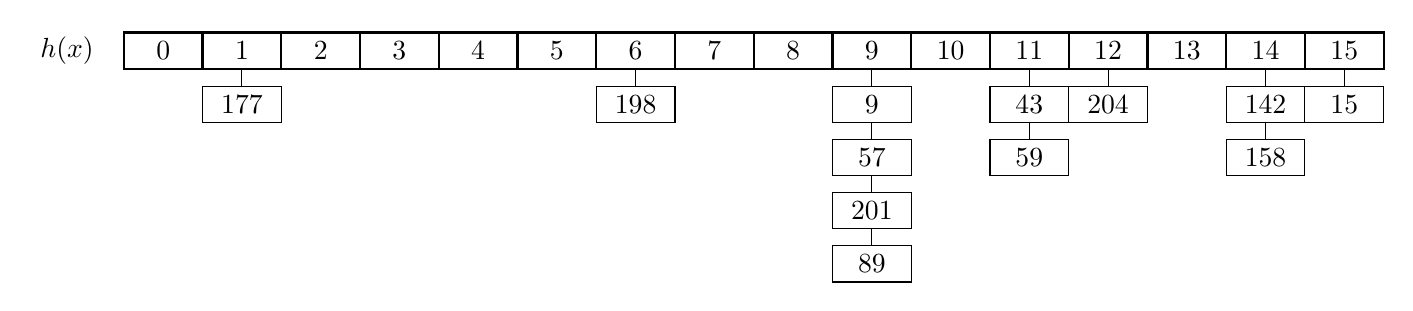
\begin{tikzpicture}[start chain=1 going right,every node/.style={draw,minimum
        width=1.0cm}] 
        \begin{scope}[node distance=-\pgflinewidth,thick]
        \foreach \X [count=\Y] in {0,...,15}
        {\node [on chain=1] (X\X) {\X};}
        \end{scope}
        \begin{scope}[node distance=2mm]

        \node[below=of X1] (Y177){177};
        \draw (X1) -- (Y177);

        \node[below=of X6] (Y198){198};
        \draw (X6) -- (Y198);

        \node[below=of X9] (Y9){9};
        \node[below=of Y9] (Y57){57};
        \node[below=of Y57] (Y201){201};
        \node[below=of Y201] (Y89){89};
        \draw (X9) -- (Y9) -- (Y57) -- (Y201) -- (Y89);

        \node[below=of X11] (Y43){43};
        \node[below=of Y43] (Y59){59};
        \draw (X11) -- (Y43) -- (Y59);

        \node[below=of X12] (Y204){204};
        \draw (X12) -- (Y204);

        \node[below=of X14] (Y142){142};
        \node[below=of Y142] (Y158){158};
        \draw (X14) -- (Y142) -- (Y158);

        \node[below=of X15] (Y15){15};
        \draw (X15) -- (Y15);



        \node[left=of X0,draw=none] (H){$h(x)$};
        \end{scope}
        \end{tikzpicture}
    \centering

    

    $(b)$ Linear Probing:

    \begin{table}[h]
        \centering
        \begin{tabular}{l|l|l|l|l|l|l|l|l|l|l|l|l|l|l|l|l|}
        \cline{2-17} 
        $h(x)$ & 0  & 1  & 2   & 3  & 4 & 5 & 6   & 7 & 8 & 9 & 10 & 11 & 12  & 13  & 14  & 15  \\ \cline{2-17} 
        $x$    & 89 & 15 & 177 & 59 &   &   & 198 &   &   & 9 & 57 & 43 & 204 & 201 & 142 & 158 \\ \cline{2-17} 
        \end{tabular}
    \end{table}



    $(c)$ Double Hashing:
    

\begin{table}[h]
    \centering
    \begin{tabular}{l|l|l|l|l|l|l|l|l|l|l|l|l|l|l|l|l|}
    \cline{2-17}
    $h(x)$ & 0   & 1   & 2 & 3  & 4 & 5  & 6   & 7  & 8 & 9 & 10 & 11 & 12  & 13  & 14  & 15 \\ \cline{2-17} 
    $x$    & 177 & 158 &   & 89 &   & 15 & 198 & 59 &   & 9 &    & 43 & 204 & 201 & 142 & 57 \\ \cline{2-17} 
    \end{tabular}
\end{table}
        
    
    \end{homeworkProblem}

    \pagebreak
    
    \begin{homeworkProblem}

    \question
    
    The \textit{text pattern matching problem} aims to find the first occurrence of a pattern string $p = p[0]p[1]...p[l-1]$ in a long document $A = A[0]A[1]A[2]...A[n-1]$.
    A simple way to solve this problem is to examine length $l$ substrings of $A$ of the form $A = A[i]A[i+1]...A[i+l-1]$ where $0 \leq i \leq n-l$ and compare them with the input pattern $p$. This procedure will take time $O(ln)$. We can improve the running time by utilising hashing. Suppose we use the hash function $h(s)=(s[0] + s[1] + ... + s[l-1]) ~ \text{mod} ~ 2^d$. 
    The procedure first computes the hash code $h(p)$. Then it compares $h(p)$ with the hash values of substrings $A[0]...A[l-1],A[1]...A[l],A[2]...A[l+1]$ and so on. 
    If we have a match of hash values, then the algorithm compares the pattern string $p$ with that substring character by character to verify the match. The algorithm returns the substring if it does matches with $p$, and it continues if the match is false. Show that this procedure can take time $O(l + n)$ plus the time spent refuting false matches.

    \answer 

    We will first consider the \textit{naive} version of this algorithm which takes $\mathcal{O}(l \cdot n)$ time. 

    Consider this piece of code (written on python) I have written:

    \begin{center}
        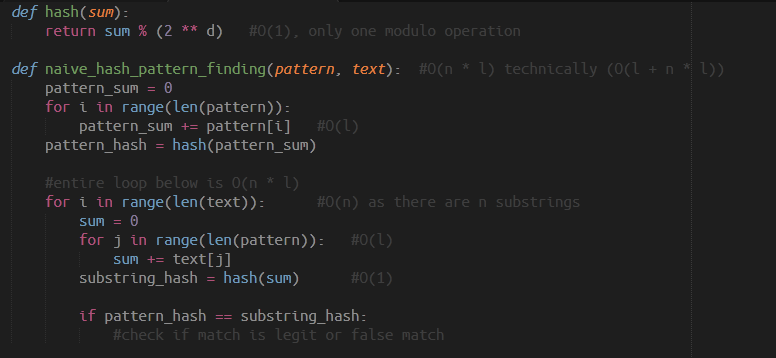
\includegraphics[scale = 0.6]{code1.png}
    \end{center}  

    Initially we have to find the hash code of the \textit{pattern} which takes $\mathcal{O}(l)$ time.
    
    Then we have to go through the text and check each possible substring and $\textit{compare}$ each possible substrings hash code with the patterns hash code (and if it is then check if the match is legitimate or false) this whole process takes around $\mathcal{O}(l \cdot n)$.

    Therefore the total complexity of this $\textit{naive}$ approach is $\mathcal{O}(l + l \cdot n) = \mathcal{O}(l \cdot n)$.

    However we can optimize this algorithm so instead of calculating of the sum of the substring every time, we take the previous sum, minus the first character of the previous substring and add the last character of our new substring:

    So consider this new piece of code:

    \begin{center}
        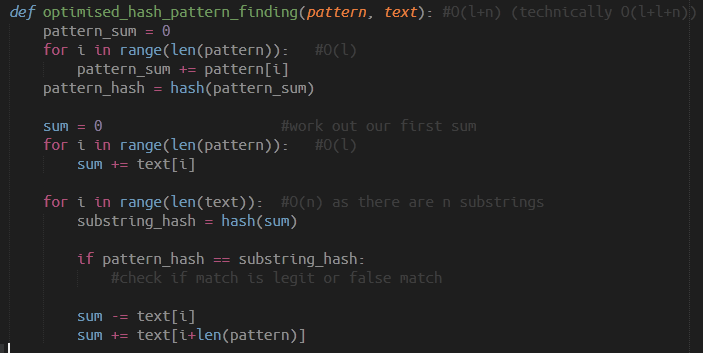
\includegraphics[scale = 0.6]{code2.png}
    \end{center}

    Initially we have to find the hash code of the \textit{pattern} which takes $\mathcal{O}(l)$ time.

    We then sum up our text (which is $l$ numbers) therefore this takes $\mathcal{O}(l)$ time.

    Now here is where we do the optimizing:

    We loop through all possible substrings in the text (which takes $\mathcal{O}(n)$ time) and get the hash code for the substring and compare it with the pattern hash code, after 
    to find the new substring sum, we minus the first character of the previous substring and add the last character of our new substring. So it is kind of like a "sliding window" (example below).

    Therefore the total time complexity of this algorithm is: $\mathcal{O}(l+l+n)=\mathcal{O}(l+n)$ plus the time taken to refute false matches.



    \textbf{We can walk through our algorithm with an example as such:}

    For example if our text was "abcdefgh" and our pattern was "def":

    We will start by finding the sum of "def" ($\mathcal{O}(l)$) and then find the hash code of "def" ($\mathcal{O}(1)$). 

    Then we find the sum of "abc" ($\mathcal{O}(l)$) and enter the loop:

    Hash the sum of "abc", compare it with the pattern hash (there is no match then move on)
    
    Find the sum and hashcode of "bcd", compare it with the pattern hash (there is no match then move on)

    Find the sum and hashcode of "cde", compare it with the pattern hash (there is no match then move on)

    Find the sum and hashcode of "def", compare it with the pattern hash (there is a match, so compare strings and return true)

    The whole process takes at most ($\mathcal{O}(n)$)

    Therefore the total time complexity is $\mathcal{O}(n+l)$ plus the time taken to refute false matches..
    
 
    \end{homeworkProblem}

    \pagebreak

    \begin{homeworkProblem}

    \question

    Chris commute by train each morning from Manukau to Britomart. $90\%$ of trains departing Manukau station on time. $80\%$ of trains arriving in Britomart on time. $75\%$ of trains depart
    on time and arrive on time.
    
    \begin{itemize}
        \item (a) Chris takes a train that departs on time. What is the probability that it will arrive on
        time?
        \item (b) Chris arrives in Britomart on time. What is the probability that his train departed on
        time?
        \item (c) Are the events, departing on time and arriving on time, independent?
    \end{itemize}

    \answer 

    We know these things from the question:

    Let events be: $A = \text{Train departing from Manukau on time}$ and $B = \text{Train arriving at Britomart ont time}$ 
    \begin{align*}
        P(A) &= 0.9 \\ 
        P(A^{c}) &= 0.1 \\
        P(B) &= 0.8 \\
        P(B^{c}) &= 0.2 \\
        P(A \cap B) &= 0.75
    \end{align*}

    (a) The question can be rephrased as: Given the situation where Chris takes a train that departs on time $(A)$, what is the probability that he will arrive on time $(B)$:

    Therefore we use the conditional probability formula: $$\boxed{P(B|A) = \frac{P(A \cap B)}{P(A)} = \frac{0.75}{0.9} = \frac{5}{6}}$$

    (b) The question can be rephrased as: Given the situation where Chris arrives at Britomart at time $(B)$, what is the probability that his train departed from Manukau on time $(A)$?
    $$\boxed{P(A|B) = \frac{P(A \cap B)}{P(B)} = \frac{0.75}{0.8} = \frac{15}{16}}$$

    (c) The test for independence is if $P(A \cap B) = P(A) \cdot P(B)$ therefore 

    Therefore since we have that $P(A \cap B)=0.75$ and $P(A) = 0.9$ and $P(B) = 0.8$ we then have that 
    $$ \boxed{P(A \cap B) = P(A) \cdot P(B) \Leftrightarrow 0.75 \neq 0.72}$$ therefore we conclude that the events departing on time from Manukau and arriving on time at Britomart are not independent.
    
    \end{homeworkProblem}


    \end{document}